\documentclass[class=article, crop=false]{standalone}
\usepackage{mathtools}
\usepackage{amsmath}
\usepackage{import}
\usepackage{float}


\setcounter{section}{0}
\begin{document}

\section{Résultats des tests}
Dans cette partie, nous allons comparer les performances de nos algorithmes implémentés:
\emph{Next-Fit(NF), Next-Fit Decreasing(NFD), First-Fit(FF), First-Fit Decreasing(\emph{FF}), Best-Fit(BF) et Best-Fit Decreasing (BFD)}. 

Pour pouvoir faire une bonne comparaison avec les autres méthodes de résolution du problème du Bin Packing,
on a trouvé judicieux de prendre les même instances du benchmark Scholl. \\

\textbf{Remarque}: les méthodes ont été développées en utilisant le langage de programmation \textbf{python}, et exécutées sur un \textbf{DELL Inspiron15 [Intel® Core™ i7-8550U CPU @ 1.80GHz×8, 8Go]}\\

Pour pouvoir comparer entre les performances des différentes méthodes heuristiques, notre étude se portera sur 2 axes:
\begin{itemize}
    \item Le temps d’exécution.
    \item La qualité de la solution.
\end{itemize}

\subsection{Analyse des résultats par rapport au temps d’exécution}
les résultats en temps d'exécution sont présentés dans le tableau suivant:  

\begin{figure}[H]
    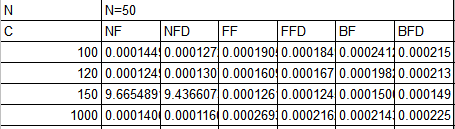
\includegraphics[width=\linewidth]{../figures/tab_part1.png}
    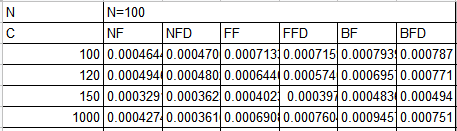
\includegraphics[width=\linewidth]{../figures/tab_part2.png}
    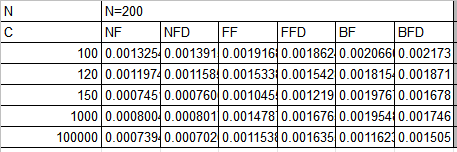
\includegraphics[width=\linewidth]{../figures/tab_part3.png}
    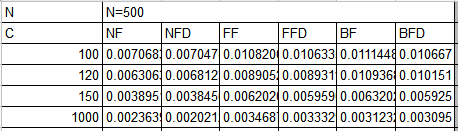
\includegraphics[width=\linewidth]{../figures/tab_part4.png}
    \caption{Tableau des temps d'exécution des heuristiques}

\end{figure}

Pour faciliter la lecture des résultats, l’utilisation d’un graphique s’impose. Ci-dessous un histogramme représentant les temps d’exécution en fonction des instances pour chaque heuristique:
\begin{figure}[H] 
    \caption{Histogramme des temps d'exécution des heuristiques}
\end{figure}

\begin{figure}[H] 
    \caption{Comparaison des temps d'exécution des heuristiques avec les méthodes exactes}
\end{figure}
\subsubsection{Analyse des résultats}
\begin{itemize}
    \item En augmentant la complexité du problème \emph{( N et C)}, le temps d'exécution des heuristiques augmente, mais tout en restant incomparable avec celui des méthodes exactes.
    \item Toutes les méthodes heuristiques arrivent rapidement à trouver une solution aux instances du problème pour les trois classes d’instances du Benchmark Scholl (moins de 0.012s).
    \item Les performances de NF et NFD sont meilleures que celles des autres méthodes, avec le BF et BFD qui consomment le plus de temps, dans la plupart du temps, pour trouver une solution.
    \item Les heuristiques \emph{FF} et \emph{FFD} s’exécutent en des temps légèrement meilleurs que BF et BFD mais moins rapides que NF et NFD.
\end{itemize}

\subsubsection{Interprétation des résultats}
\begin{itemize}
    \item Les algorithmes BF et BFD nécessitent plus de temps car le principe de BF repose sur le fait qu’il faut d’abord parcourir toutes les boîtes déjà ouvertes avant de prendre une décision (ranger un article).
    \item Les algorithmes NF et NFD sont les plus rapide car le principe de NF repose sur le fait que la décision où mettre l’article concerne seulement la dernière boîte ouverte, donc on n’a pas à parcourir l’ensemble des boîtes pour chaque article.
    \item Les algorithmes \emph{FF} (resp \emph{FFD}) impose de parcourir partiellement la liste des boîtes ouvertes jusqu’à trouver la 1ère boîte qui convient, ce qui justifie le temps d’exécution moyen ( entre celui de BF et NF).
\end{itemize}

\subsection{Analyse des résultats par rapport à la qualité de la solution}
Pour cela, on utilisera la métrique Worse case Ratio \textbf{[ voir Chapitre 02]} \\

\textbf{Remarque:} 
Vu que les instances du benchmark Scholl contiennent des articles déjà ordonnés, les versions \emph{online (NF,FF,BF)} et \emph{offline (NFD, \emph{FF},BFD)} des heuristiques donnent exactement les même résultats ( car la différence entre les deux c’est l’étape d’ordonnancement des articles ). Dans cette partie nous allons nous contenter d’étudier la qualité de la solution des algorithmes \emph{onlines}.\\

Ci-dessous un tableau récapitulatif des ratios obtenus pour chaque heuristique sur l’ensemble des instances du benchmark \textbf{[figure x]} , ainsi qu’une représentation graphique ( en histogramme) de ces résultats \textbf{[figure xx]}:

\begin{figure}[H]
    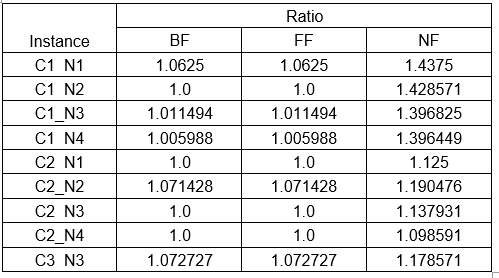
\includegraphics[width=\linewidth]{../figures/tab_ratio_heur.png}
    \caption{Tableau des ratios obtenues par les heuristiques}
\end{figure}

\begin{figure}[H] 
    \caption{Histogramme des ratios des heuristiques en fonction des instances}
\end{figure}

Ci-dessous une représentation graphique (en histogramme) qui représente le ratio de toutes les instances du Benchmark \emph{Scholl}, toutes classes confondues par heuristique (BF,FF et NF): 

\begin{figure}[H] 
    \caption{Histogramme des ratios des heuristiques pour tout le benchmark Scholl}
\end{figure}

\subsubsection{Analyse des résultats}
\begin{itemize}
    \item Les ratios obtenus pour \emph{BF} et \emph{FF} (\emph{BFD} et \emph{FF} resp) sont identiques et diffèrent de \emph{NF (NFD)}.
    \item Les heuristiques \emph{BF, FF} (et respectivement \emph{BFD}, \emph{FF}) arrivent pour certains types d’instances à trouver la valeur optimales du problème (ratio égale 1), contrairement à \emph{NF} (respectivement \emph{NFD}) qui ne trouve pas assez souvent la solution (ratio supérieure à 1).
\end{itemize}

\subsubsection{Interprétation des résultats}

\subsection{Conclusion}
En exécutant les heuristiques étudiées ( \emph{FF, NF ,BF} et leurs versions \emph{offline}) sur les instances du benchmark Scholl, on a trouvé que l’heuristique NF est la plus rapide à s’exécuter, mais elle donne la plus mauvaise qualité de solution. Par contre les heuristiques \emph{FF} et \emph{BF} sont moins rapides ( avec \emph{BF} légèrement moins rapide que \emph{FF} )  mais offrent une meilleure qualité.  

Comme on a pu le constater durant ce chapitre, les méthodes heuristiques de type \emph{online (FF, NF,BF)} et de type \emph{offline (FF, NFD, BFD)} donnent de très bon résultats par rapport au temps d’exécution. Mais l’un des inconvénient avec les méthodes heuristiques c’est qu’elles n'assurent pas la qualité de la solution.

Ces algorithmes sont connu sous le nom d’algorithmes gloutons, c’est à dire qu’ils cherchent à trouver une solution dans un temps très réduit, mais ne donne pas d’assurance sur la qualité de cette solution. C’est pour cela que ces méthodes sont généralement utilisées pour initialiser d’autres méthodes plus sophistiquées comme les métaheuristiques.


\end{document}